\documentclass[tikz,border=5pt]{standalone}
\usepackage{lmodern}
\renewcommand{\familydefault}{\sfdefault}
\usetikzlibrary{arrows.meta,calc}
% Training-recipe figures: match Ch 3's rlhf-basic.png / rlhf-complex.png.
% Latin Modern Sans, unfilled-looking boxes, gray open arrowheads, soft elbows.
% Requires \usetikzlibrary{arrows.meta,calc} and \usepackage{lmodern}.
% Compile with \def\figdark{1} for the site's slate dark theme.
\providecommand{\figdark}{0}
\ifnum\figdark=1
  \definecolor{recipebackground}{HTML}{1E293B}
  \definecolor{recipeborder}{HTML}{CBD5E1}
  \definecolor{recipetext}{HTML}{CBD5E1}
  \definecolor{recipearrow}{HTML}{94A3B8}
\else
  \definecolor{recipebackground}{HTML}{FFFFFF}
  \definecolor{recipeborder}{HTML}{262626}
  \definecolor{recipetext}{HTML}{333333}
  \definecolor{recipearrow}{HTML}{A6A6A6}
\fi

\tikzset{
  recipe model/.style={
    rectangle, rounded corners=2pt,
    draw=recipeborder, fill=recipebackground, text=recipetext,
    line width=1.05pt,
    minimum width=2.8cm, minimum height=0.95cm,
    inner xsep=7pt, inner ysep=5pt,
    font=\fontsize{14}{17}\selectfont, align=center
  },
  recipe line/.style={
    draw=recipearrow, line width=1.4pt,
    line cap=round, line join=round, rounded corners=7pt
  },
  recipe arrow/.style={
    recipe line,
    -{Straight Barb[length=2.7mm,width=4.2mm]}, shorten >=5pt
  },
  recipe label/.style={
    text=recipetext, font=\fontsize{10}{13}\selectfont,
    align=center, inner sep=2pt
  },
  recipe operation/.style={recipe label, font=\fontsize{10}{13}\selectfont\itshape},
  recipe edge operation/.style={recipe operation, anchor=south, yshift=5pt},
  recipe example/.style={
    recipe label, font=\fontsize{8.5}{10}\selectfont,
    anchor=north, inner sep=0pt, yshift=-3pt
  }
}


% Generic sequential-RL pattern, using the stage order of the supplied GLM-5
% slide/report. Boxes are model checkpoints; edge labels are training stages,
% as in Ch 3's existing rlhf-basic.png and rlhf-complex.png figures.
% This shows the sequential RL spine, not GLM-5's complete recipe: its final
% on-policy cross-stage distillation is omitted. No GLM-5.2-specific claim.
% Sources and deliberate simplifications: see this directory's README.md.
\begin{document}
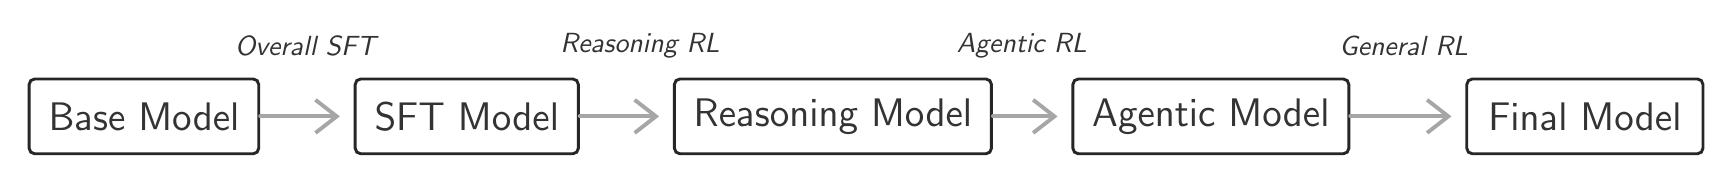
\begin{tikzpicture}
  \node[recipe model] (base) at (0,0) {Base Model};
  \node[recipe model] (sft) at (4.1,0) {SFT Model};
  \node[recipe model,minimum width=3.25cm] (reasoning) at (8.75,0) {Reasoning Model};
  \node[recipe model,minimum width=3.25cm] (agentic) at (13.55,0) {Agentic Model};
  \node[recipe model,minimum width=3cm] (final) at (18.3,0) {Final Model};

  \draw[recipe arrow] (base.east) -- (sft.west);
  \draw[recipe arrow] (sft.east) -- (reasoning.west);
  \draw[recipe arrow] (reasoning.east) -- (agentic.west);
  \draw[recipe arrow] (agentic.east) -- (final.west);
  \node[recipe operation] at (2.05,0.9) {Overall SFT};
  \node[recipe operation] at (6.3,0.9) {Reasoning RL};
  \node[recipe operation] at (11.15,0.9) {Agentic RL};
  \node[recipe operation] at (16,0.9) {General RL};
\end{tikzpicture}
\end{document}
